The utility of interactive visualizations depends on the ability of users to create them. Typically, data scientists or analysts work in teams. Contributions are made from every person on the team, and then the team must present their findings in a non-exploratory context. Sometimes it is useful to be able to show the path of exploration that the team has taken, using some kind of history model. This chapter presents an approach to enabling all of the above features, leveraging reactive models.

\section{Related Work}
Several projects have focused explicitly on visualization of public data on the Web. ManyEyes was an experiment in scaling the audience for visualizations by empowering users to create visualizations of their own data \cite{viegas2007manyeyes}. ManyEyes provided a fixed set of pre-packaged visualization tools and allowed users to visualize their own data tables using the provided visualizations. GapMinder is a project aimed at exposing public data (primarily the United Nations Millenium Development Goals Indicators) using visualization \cite{rosling2005new}. GapMinder includes an animated scatter plot with an interactive time slider, a line chart showing statistics over time, and a world map (see figure \ref{fig:gapminder}). The Google Public Data Explorer provides a visual interface to selected public data sets similar to GapMinder, but it does not make the data available to users in machine-readable form \cite{googlePublicDataExplorer}.

\begin{figure}[h!]
  \centering
  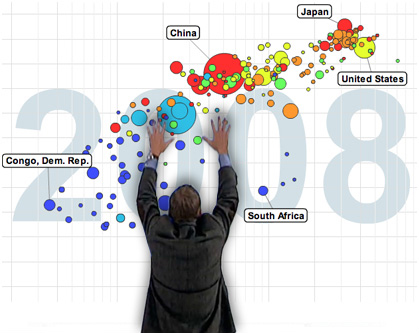
\includegraphics[width=\figureWidth]{figs/gapminder.jpg}
  \caption[GapMinder and Hans Rosling.]
   {GapMinder, a public data visualization tool based on an animated scatter plot, timeline, and map. Here, Professor Hans Rosling, the creator of GapMinder, is shown gesturing the motion of the plot while presenting the visualization.}
  \label{fig:gapminder}
\end{figure}
\pagebreak

Many data visualization and analysis tools have been developed with collaboration in mind. Tableau Server has collaboration features such as sharing visualizations, commenting on visualizations, embedding visualizations in Web pages, and sharing filtered data. The OpenChorus project supports annotation and sharing of data sources using a variety of database technologies including SQL, Hadoop (HDFS), Oracle, and Greenplum \cite{openChorus}. Foundational collaboration technologies include Operational Transform for synchronous collaboration such as Google Docs \cite{sun1998operational} and revision control systems for asynchronous collaboration such as GitHub \cite{o2009making, dabbish2012social}.

\section{Application State Model}
An application typically consists of instantiations of many reusable components. For example, an AngularJS application instantiates reusable components encapsulated as Angular directives, and a BackboneJS application instantiates Views for specific Models.

Interactive visualizations with multiple linked views share common patterns, including layout based on nested boxes and view linkage based on flows between interaction output, data transformations, and visualization input. This configuration can be expressed as a set of reactive models. Some models, such as the layout and linkages, must be able to access other models in the system and change their properties (e.g., the bounding box for layout and the selected elements for linked views). A simple structure based on named models can accommodate the above needs.

Our application state structure consists of \emph{components}, each of which has:
\begin{itemize}
\item \emph{alias} The string identifier for the component.
\item \emph{module} The string that defines which module to instantiate.
\item \emph{model} A collection of serialized model properties.
\end{itemize}

This structure can be serialized using JSON \cite{crockford2006application}. The overall application state configuration is an object whose keys are component aliases, and whose values are component objects. Each component object contains key-value pairs representing its serialized model state. Each component also has a value for the \verb1module1 property that determines which module is invoked to instantiate the component at runtime. Figure \ref{fig:dashboardLayout} shows an example of a configuration that instantiates simple components into a nested box layout. This layout technique is one of the foundations for assembling linked views. Any reusable visualization can be placed into a box in the layout, then linked with other visualizations within the same layout. Figure \ref{fig:prototype} shows an example nested box layout that includes visualizations.

\begin{figure}
  \centering
  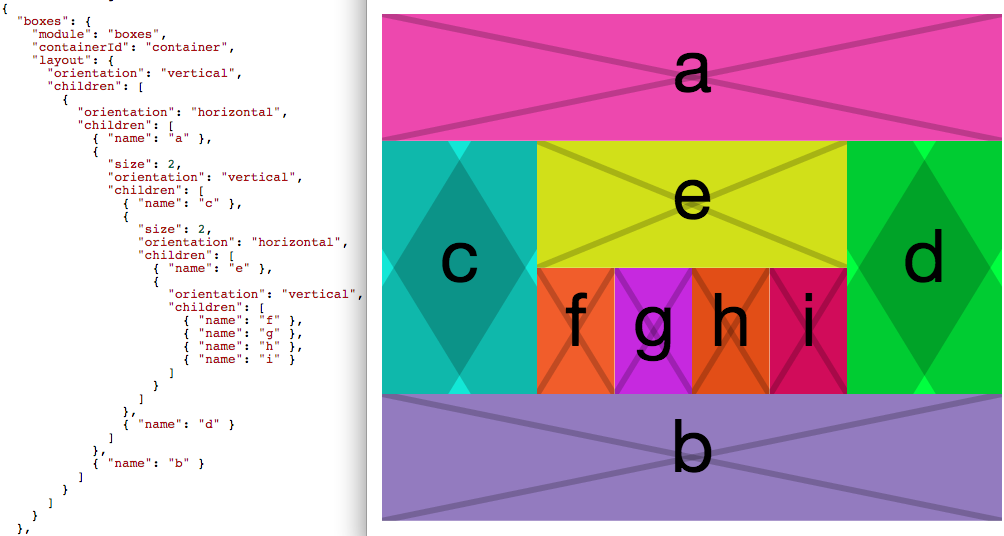
\includegraphics[width=\figureWidth]{figs/boxes.png}
  \caption [Nested Box Layout Configuration]{An example configuration that defines a nested box layout. }
  \label{fig:dashboardLayout}
\end{figure}

\begin{figure}
  \centering
  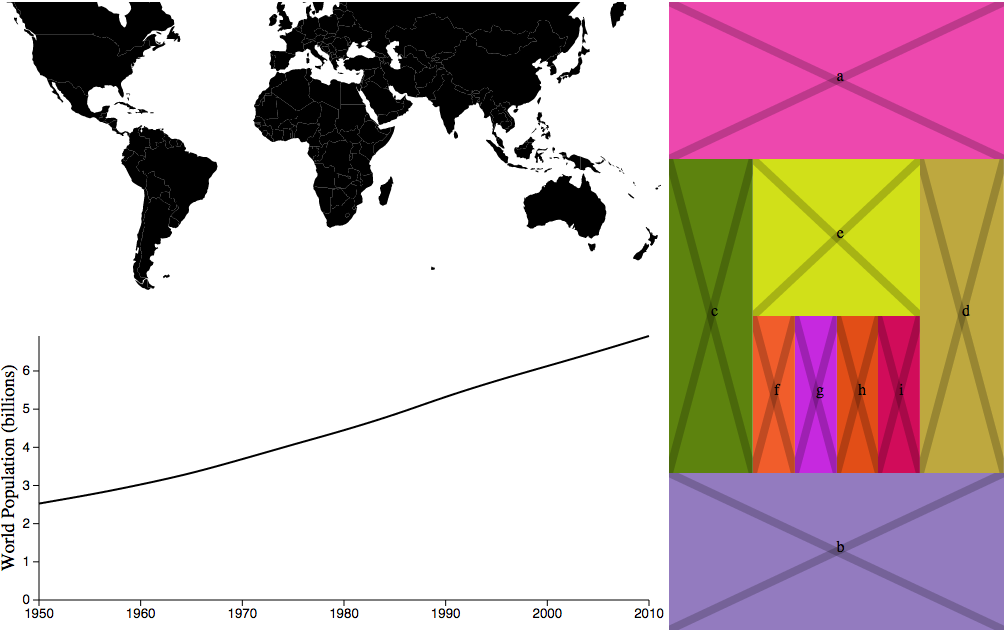
\includegraphics[width=\figureWidth]{figs/prototype.png}
  \caption [Nested Boxes with Visualizations]{An example configuration that defines a nested box layout including line chart and map visualizations. }
  \label{fig:prototype}
\end{figure}

\section{Runtime Engine}
The application state model addresses the configuration and serialization structure of the application state. A runtime model is necessary to transform serialized application state models into a running system. The runtime engine performs this transformation as follows:

\begin{itemize}
\item The runtime engine module loader is instantiated. This process defines a mapping from module names to constructor functions that instantiate the components, returning reactive models.
\item The \verb`module` property of each component in the application state configuration is used to instantiate each component.
\item The runtime engine maintains a dictionary whose keys are component aliases and whose values are instantiated components.
\item Instantiated components can request references to other instantiated components from the runtime. This operation must be asynchronous to account for dynamic module loading.
\end{itemize}

As an example, consider the flow of instantiation for the application state shown in figure \ref{fig:dashboardLayout}. The runtime uses the \verb1module1 property on each component to fetch and invoke its constructor module. The \verb`boxes` module computes the nested box layout. The computed nested box layout is used for dynamically positioning and sizing the interactive visual components.

The first prototype of the interactively configurable runtime engine was developed during a summer internship at Rapid7, a cybersecurity company, to create an interactive visualization dashboard with multiple linked views for analyzing corporate login activity. Technologies used for visualization included D3.js, a visualization framework that uses SVG, and Leaflet.js, a framework for geographic maps. The map showed where users have logged into the network, aggregated geographically using the Leaflet MarkerCluster plugin and visualized using D3's Pie Chart layout. Black represented successful logins and blue represented failed logins. This industry application of our dashboard layout framework demonstrates its capability to define dashboards with multiple linked views. The resulting visualization dashboard is shown in figure \ref{fig:ingressDash}.

\begin{figure}
  \centering
  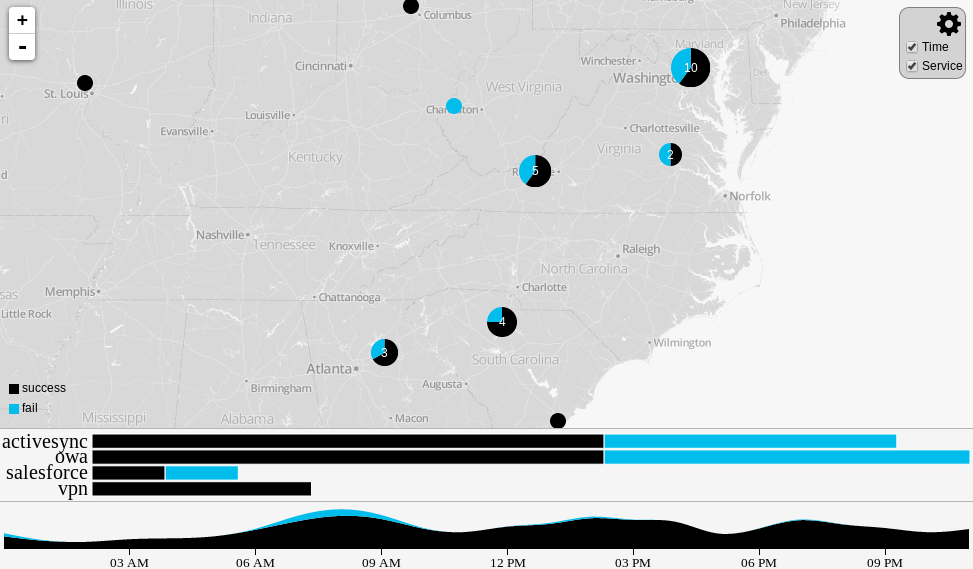
\includegraphics[width=\figureWidth]{figs/mapDocs7.png}
  \caption[The Rapid7 Ingress Dashboard.]
   {This visualization dashboard shows corporate login data and is integrated into the Rapid7 product called UserInsight.}
  \label{fig:ingressDash}
\end{figure}

\begin{figure}
  \centering
  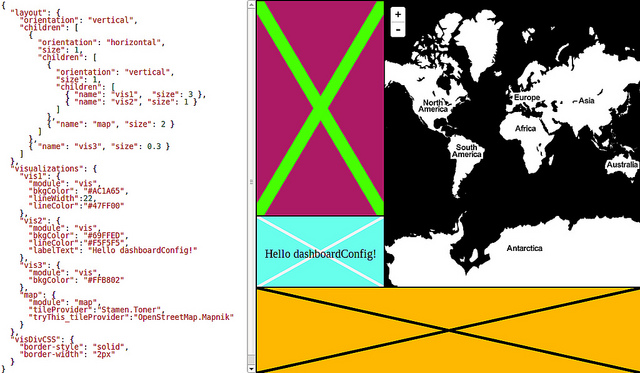
\includegraphics[width=\figureWidth]{figs/dashboardScaffold.png}
  \caption[Dashboard Scaffold Configuration Editor.]
   {The dashboard scaffold prototype, showing an interactive text-based configuration editor on the left, and a sample dashboard on the right. This shows how Leaflet-based maps can be integrated with D3 visualizations using the proposed configuration framework.}
  \label{fig:ingressDash}
\end{figure}

\section{Changing State}
When the application state configuration changes, the runtime components must be updated accordingly. Consider the scenario of a user manually editing the application state configuration using a text editor. Every time the user changes the configuration, the system must update the runtime to reflect the new configuration. A na\"{\i}ve approach to this problem is to tear down and re-instantiate the entire runtime whenever the configuration changes. This approach, while functionally correct, does an extraordinary amount of unnecessary work. A more efficient solution would employ a strategy in which only the changes in configuration are propagated through the runtime, while unchanged configuration parameters need not have any effect on the runtime.

All application state configuration updates can be expressed as a series of the following operations:
\begin{itemize}
\item create(alias, module)
\item destroy(alias)
\item set(alias, property, value)
\item unset(alias, property)
\end{itemize}

In the context of a user manually updating the configuration at runtime, the difference between two configurations can be computed. The difference results in a structure that can be applied to the runtime essentially as a patch.

\section{Real-time Synchronization}
While Operational Transform algorithms address the general case of many-way synchronization for arbitrary text \cite{cormack1995counterexample}, if we have a simpler application state configuration structure, it is possible to implement simpler many-way synchronization algorithms. Our simple application state configuration difference structure provides an important primitive for real time configuration. The configuration difference objects computed locally can be broadcast to other clients and applied to remote runtimes to achieve real time many-way synchronization.

To implement real time synchronization, consider the application state and its changes as a directed graph $G = (V, E)$. Vertices in the graph represent application states, and each directed edge between nodes $u$ and $v$ represents a change in state. In a distributed environment with multiple clients, any client can originate a new state. The client that creates a new state provides the associated configuration difference object that can move any client runtime from state $u$ to state $v$ when applied.

Situations may arise in which the source state $u$ of a new state transition does not match the current runtime state. This occurs when two or more clients simultaneously originate conflicting state changes. The distributed synchronization algorithm must guarantee that no matter which order the conflicting state transitions arrive at the server, all clients must ultimately end up in the same state. This requirement can be implemented with simple algorithms that throw away some changes, or more complex algorithms that preserve every change.

Simple distributed synchronization algorithms can be developed that implement either ``first one wins'' or ``last one wins'' semantics. First one wins semantics means that the first of several conflicting state transitions that arrives at the server is accepted as the authoritative one and forced upon clients, causing the clients to roll back local conflicting changes. Last one wins semantics means that the last of several conflicting state transitions that arrives at the server is accepted as the authoritative one, causing the server to compute rollbacks and broadcast them to clients. Either way, clients experience loss of changes. In use cases with many concurrent users making changes simultaneously, these semantics would lead to frustrating user experiences, as users must perform their actions twice or more before they are accepted into the authoritative state.

%TODO include pseudocode and diagrams for first one wins and last one wins semantics

More complex algorithms that involve merging conflicting state transitions can address multiple concurrent changes. These algorithms must merge multiple configuration difference objects and generate a new state originating at the server. The server, with awareness of the states of each client, must send different transitions to each client such that each client ultimately is in the new state that originated from the server.

%TODO include pseudocode and diagrams for merge

\section{History Model}
Using the state machine model discussed, transitions can be annotated with an undo operation to enable history graph navigation. Each transition that occurs in the system adds a forward edge (a ``do'' operation) and a backward edge (an ``undo'' operation) to the history graph. Numerous algorithms exist for computing the shortest path in an arbitrary directed graph \cite{gallo1988shortest}. A shortest path algorithm such as Dijkstra's can be used to compute the sequence of configuration difference objects to apply to a runtime in order to transition the system from any state to any other state.

\section{Integration with Web Technologies}
To build interactive visualizations for the Web using reactive models, there must be a clearly defined way to interface between reactive models and Web graphics technologies. The primary Web graphics technologies are Canvas and SVG (Scalable Vector Graphics). The Canvas element provides an additional API called WebGL that supports hardware accelerated graphics. The goal of integrating reactive models with Web graphics technologies is to build reusable interactive graphics modules. The modules can be instantiated and linked with specific data to create interactive visualizations.

Instantiations of reusable interactive graphics components in general function in conjunction with a DOM element. Therefore, one way to accommodate any Web technology is to design an API in which a module constructor function creates a DOM element that contains its visual representation. Cascading Style Sheets (CSS) can then be used to position the DOM element. This approach effectively unifies Canvas, WebGL, and SVG, and allows interactive graphics modules authored using different APIs to function together on a single page.

